% Asset ID: AS1CoordinateGeometryCirclesTikZ-005
% Purpose: Show tangent perpendicular to radius.
\documentclass[tikz,border=8pt]{standalone}
\usetikzlibrary{calc}
\begin{document}
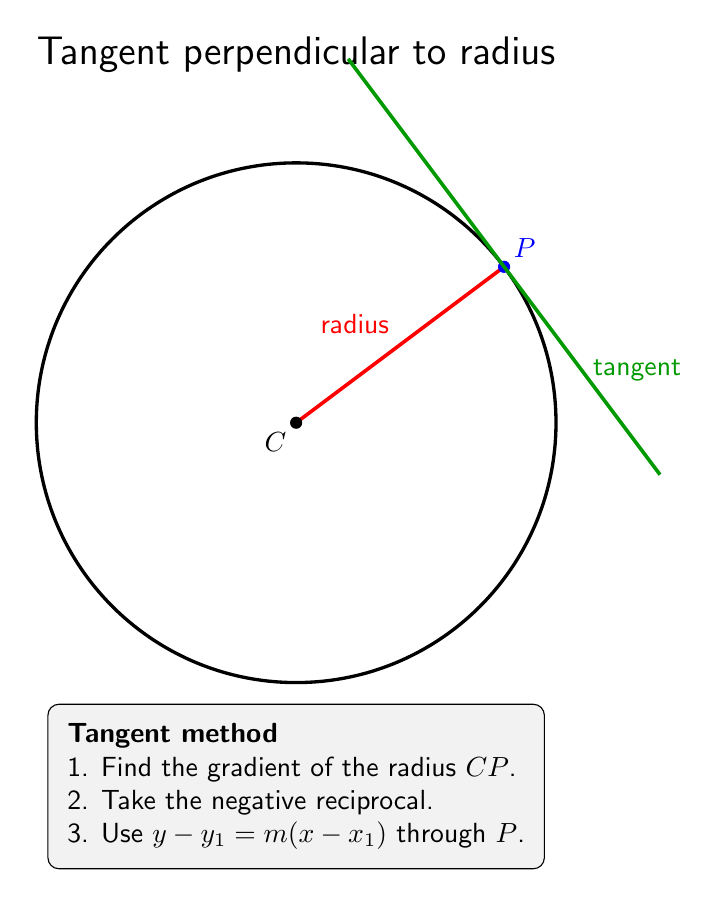
\begin{tikzpicture}[scale=1.1, font=\sffamily]
\node[align=center] at (0,4.25) {\Large Tangent perpendicular to radius};
\coordinate (C) at (0,0); \draw[line width=1.2pt] (C) circle (3); \coordinate (P) at (2.4,1.8);
\draw[line width=1.3pt, red] (C)--(P) node[midway, above left] {radius}; \fill[black] (C) circle (2pt) node[below left] {$C$}; \fill[blue] (P) circle (2pt) node[above right] {$P$};
\coordinate (T1) at ($(P)+(-1.8,2.4)$); \coordinate (T2) at ($(P)+(1.8,-2.4)$); \draw[line width=1.3pt, green!60!black] (T1)--(T2) node[near end, right] {tangent};
\node[align=left, draw, rounded corners, fill=gray!10, inner sep=7pt] at (0,-4.2) {\textbf{Tangent method}\\1. Find the gradient of the radius $CP$.\\2. Take the negative reciprocal.\\3. Use $y-y_1=m(x-x_1)$ through $P$.};
\end{tikzpicture}\end{document}
